\begin{titlepage}
\addcontentsline{toc}{chapter}{Title Page}

\begin{center}

%% Extra whitespace at the top.
\vspace*{2\bigskipamount}

%% Print the title.
{\makeatletter
\bfseries\LARGE{Ultrafast quantum dynamics of doped superfluid helium nano-droplets}
\makeatother}

%% Print the optional subtitle.
{\makeatletter
\ifx\@subtitle\undefined\else
    \bigskip
    \titlefont\titleshape\Large\@subtitle
\fi
\makeatother}

\end{center}

\cleardoublepage
\thispagestyle{empty}

\begin{center}

%% The following lines repeat the previous page exactly.

\vspace*{2\bigskipamount}

%% Print the title.
{\makeatletter
\bfseries\Huge\textsc{\textcolor{activeColor}{Ultrafast quantum dynamics of doped superfluid helium nano-droplets}}
\makeatother}

%% Print the optional subtitle.
{\makeatletter
\ifx\@subtitle\undefined\else
    \bigskip
    \titlefont\titleshape\Large\@subtitle
\fi
\makeatother}

%% Uncomment the following lines to insert a vertically centered picture into
%% the title page.
\vfill
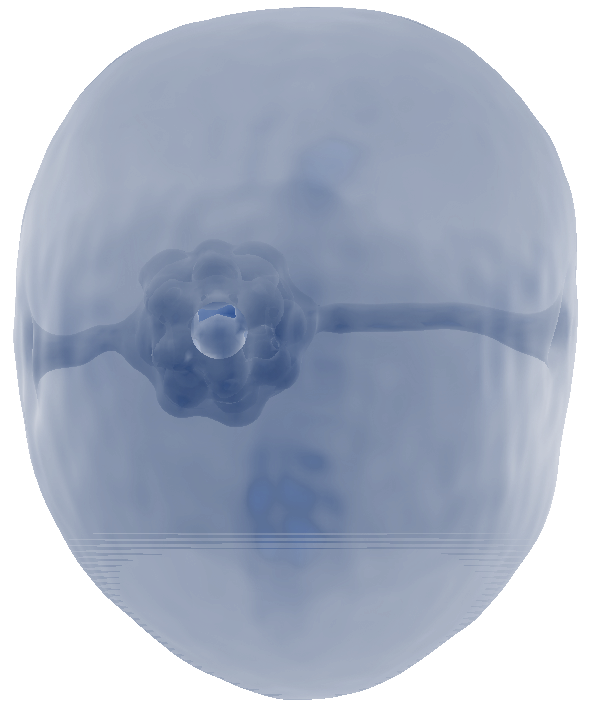
\includegraphics[height=6.5cm]{title}
\vfill

%% Apart from the names and dates, the following text is dictated by the
%% promotieregelement.

{\Large\bfseries\textsc{\textcolor{activeColor}{Th\`{e}se}}}

\bigskip
\bigskip

en vue de l'obtention du doctorat de l'université de Toulouse,

délivré par l'Université Toulouse III Paul Sabatier (UT3 Paul Sabatier),

présentée et soutenue le mardi 29 mars 2018 à 10h30

\bigskip
\bigskip

par

\bigskip
\bigskip

%% Print the full name of the author.
\makeatletter
{\Large\bfseries\textsc{François M.G.J. Coppens}}
\makeatother

\bigskip
\bigskip

Né à Roosendaal en Nispen, Pays-Bas

%% Extra whitespace at the bottom.
\vspace*{2\bigskipamount}

\end{center}

\clearpage
\thispagestyle{empty}

%% The following line is dictated by the promotieregelement.
\noindent Dit proefschrift is goedgekeurd door de

%% List the promotors (supervisors).
\medskip\noindent
\begin{tabular}{l}
    promotor: prof.\ dr.\ A.\ Kleiner \\
    copromotor: dr.\ A.A.\ Aaronson
\end{tabular}

\bigskip
\noindent Samenstelling promotiecommissie:

%% List the committee members, starting with the Rector Magnificus and the
%% promotor(s) and ending with the reserve members.
\medskip\noindent
\begin{tabular}{p{3cm}l}
    Rector Magnificus, & voorzitter \\
    Prof.\ dr.\ A.\ Kleiner, & Technische Universiteit Delft \\
    Dr.\ A.A.\ Aaronson, & Technische Universiteit Delft \\

    \medskip
    \mbox{\emph{Onafhankelijke leden:}} & \\

    Prof.\ dr.\ A.\ Jansen & Technische Universiteit Delft \\
    % Special case, only for very long names
    \mbox{Prof.\ dr.\ ir.\ A.B.C.D.\ van de Lange-Achternaam} & \\
      & Technische Universiteit Delft \\
    Prof.\.dr.\ N.\ Nescio & Politecnico di Milano, Itali\"e \\
    Prof.\ dr.\ ir.\ J.\ Doe, & Technische Universiteit Delft, reservelid \\

    \medskip
    \mbox{\emph{Overige leden:}} & \\
    Prof.\ dr.\ ir.\ J.\ de Wit, & Technische Universiteit Delft \\
    Dr.\ ir.\ Q.\ de Zwart, & Technische Universiteit Eindhoven \\
\end{tabular}

%% Include the following disclaimer for committee members who have contributed
%% to this dissertation. Its formulation is again dictated by the
%% promotieregelement.
\medskip
\noindent Prof.\ dr.\ ir.\ J.\ de Wit heeft in belangrijke mate aan de totstandkoming van het proefschrift bijgedragen.

%% Here you can include the logos of any institute that contributed financially
%% to this dissertation.
\vfill
%\begin{center}
%    \includegraphics[height=0.5in]{title/logos/tudelft}
%    \hspace{2em}
%    \includegraphics[height=0.5in]{title/logos/casimir} \\
%    \includegraphics[height=0.5in]{title/logos/fom}
%    \hspace{2em}
%    \includegraphics[height=0.5in]{title/logos/nwo}
%\end{center}
\vfill

\noindent
\begin{tabular}{@{}p{0.2\textwidth}@{}p{0.8\textwidth}}
    \textit{Keywords:} & \ldots \\[\medskipamount]
    \textit{Printed by:} & Fran\c{c}ois Coppens \\[\medskipamount]
    \textit{Front \& Back:} & Beautiful cover art that captures the entire content of this thesis in a single illustration.
\end{tabular}

\vspace{4\bigskipamount}

\noindent Copyright \textcopyright\ 2018 by F.~Coppens

%% Uncomment the following lines if this dissertation is part of the Casimir PhD
%% Series, or a similar research school.
%\medskip
%\noindent Casimir PhD Series, Delft-Leiden 2015-01

\medskip
\noindent ISBN 000-00-0000-000-0

\medskip
\noindent An electronic version of this dissertation is available at \\
\url{http://repository.tudelft.nl/}.

\end{titlepage}